\chapter{Collision Detection}
\label{ch:CollisionDetection}
To provide a plausible accurate collision handling, it is essential to determine all colliding elements. Information about occurring collisions are provided by a collision detection algorithm.

We will present two different algorithms for computing intersections between triangle meshes. We first introduce a discrete collision test which tests for collisions at one moment in the time step. Afterwards, we extend the algorithm to a continuous formulation, by taking the feature trajectories into account. Thereby, we do not miss any collisions and additionally provide the contact times which are required for the CPF algorithm. Finally, we have a look at how the collision detection can be sped up with bounding volume hierarchies.

\section{Broad and Narrow Phase}
To check two bodies for intersections with elementary collision tests requires to test each element of the first body against all elements of the second body. Therefore, it scales in $O(nm)$ with $n$ and $m$ corresponding to the numbers of the surface vertices of the objects.
Since the amount of necessary tests is huge and performing all of them is expensive, most collision detections are divided into two stages.
The first stage, called "Broad Phase", uses a fast method to narrow the possibly colliding feature pairs down.
The second stage, called "Narrow Phase" applies an elemental test only to the remaining feature pairs.
The division in these two steps provides a significant speed-up \cite{BENDER2007}. In this thesis only a narrow phase is used.
\section{Discrete Collision Detection}
\label{sec:DCD}
An elementary discrete collision detection (DCD) test is to test for triangle-triangle collisions \cite{MOLLER1997}, which can be reduced to edge-triangle tests (based on \cite{Akenine-Moller2002}). All triangles of a body $A$ are tested against the edges of a body $B$ and vice versa. For a triangle $T$ with the vertices $\mathbf a$, $\mathbf b$ and $\mathbf c$, the plane $t$ defined by the triangle $T$ can be expressed as
\begin{equation}
t(\omega_b,\omega_c)=(1-\omega_b-\omega_c)\mathbf a +\omega_b \mathbf b + \omega_c \mathbf c,
\end{equation}
with the parameters $\omega_b$ and $\omega_c$ corresponding to the barycentric coordinates.

For an edge $E$ with the vertices $\mathbf p$ and $\mathbf q$ the line $e$ defined by the edge $E$ is
\begin{equation}
e(\omega_q)=\mathbf{p}+\omega_q (\mathbf{q}-\mathbf{p}),
\end{equation}
with the parameter $\omega_q$ corresponding to the barycentric coordinate.
The edge $E$ and the triangle $T$ collide if and only if $\exists \omega_q,\omega_b,\omega_c \in [0,1] \text{ such that}$
\begin{gather}
\label{eq::dcd-tv}
\mathbf{p}+\omega_q(\mathbf{q}-\mathbf{p})=(1-\omega_b-\omega_c)\mathbf a +\omega_b \mathbf b + \omega_c \mathbf c.
\end{gather}
If there exists a solution to the linear system \ref{eq::dcd-tv}, the plane and the line intersect. To ensure that the intersection is in the edge interval of the line, $ \omega_q$, $\omega_b$ and $ \omega_c$ need to be in the interval $[0,1]$.

To solve equation \ref{eq::dcd-tv} we transform it into a matrix formulation
\begin{equation}
	\mathbf{p}-\mathbf{a}=\begin{pmatrix}
	\mathbf{p}-\mathbf{q} \
	\mathbf b -\mathbf a \
	\mathbf c -\mathbf a
	\end{pmatrix}
	\begin{pmatrix}\omega_q\\\omega_b\\\omega_c
	\end{pmatrix}
\end{equation}
which can be solved using Cramer's rule.

\section{Continuous Collision Detection}
\label{sec:CCD}
Continuous collision detection (CCD) algorithms do not only detect whether two features are colliding but also when they are colliding, which is a property required by the CPF algorithm.
 Most CCD algorithms approximate the motion linearly, as described by Provot \cite{PROVOT1997}, but higher order formulations are also possible and provide a more accurate estimation of the collision times.
 
 For triangle meshes there are only two possible elementary collisions. Either a vertex goes through a triangle face resulting in a vertex-face (VF) collision or an edge goes through another edge resulting in an edge-edge (EE) collision, as shown in figure \ref{fig::asd}.

 
 We now describe how to compute collisions for both cases.
\begin{figure}[h!] 
\begin{minipage}[b]{0.5 \linewidth}
		\centering
		\subfigure[Vertex-face case]{
			       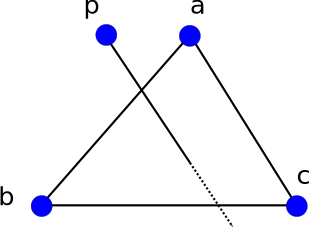
\includegraphics[width=0.5\linewidth]{pics/pdf/ccd_vf.pdf} }
	\end{minipage}
	\begin{minipage}[b]{0.5 \linewidth}
		\centering
		\subfigure[Edge-edge case]{
			       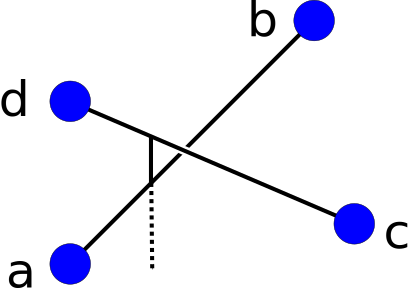
\includegraphics[width=0.5\linewidth]{pics/pdf/ccd_ee.pdf} }
	\end{minipage}

  \caption{Illustration of the possible feature pairs, VF and EE, for CCD.}
  \label{fig::asd}
\end{figure}

\paragraph{Vertex-Face}
For a moving vertex $\mathbf p(t)$ and a moving triangle $T$ with the vertices $\mathbf a(t)$, $\mathbf b(t)$ and $\mathbf c(t)$ the constant velocities associated to the linear motion are denoted as $\mathbf v_p$, $\mathbf v_a$, $\mathbf v_b$ and $\mathbf v_c$. For $t$ in the interval $[t_0,t_0+\Delta t]$, the vertex trajectories are $\mathbf p(t)=\mathbf p_0+t\mathbf v_p$, $\mathbf a(t)=\mathbf a_0+t\mathbf v_a$, $\mathbf b(t)=\mathbf b_0+t\mathbf v_b$ and  $\mathbf c(t)=\mathbf c_0+t\mathbf v_c$. The plane $f(t)$ defined by the triangle $T$ at the time $t$ can be expressed as
\begin{equation}
f(\omega_b,\omega_c,t)=(1-\omega_b-\omega_c)\mathbf a(t) +\omega_b \mathbf b(t) + \omega_c \mathbf c(t).
\end{equation}
The vertex $\mathbf p(t)$ and the triangle $T$ collide, if at one point in the time step $\mathbf p(t)$  is within $T$, which holds if and only if $\exists t \in [t_0,t_0+\Delta t], \; \exists \; \omega_b, \omega_c \in [0,1], \; \omega_b+\omega_c\le1 \text{ such that}$
\begin{gather}
\label{eq::ccd-vf}
\mathbf p_0+t\mathbf v_p=(1-\omega_b-\omega_c)\mathbf a(t) +\omega_b \mathbf b(t) + \omega_c \mathbf c(t).
\end{gather}
In contrast to the DCD the resulting equation system is non linear due to the new time dependency.
Therefore, we introduce the additional condition that at the time of collision, the vertex $\mathbf p(t)$ is coplanar to the triangle $T$. The additional condition is satisfied if $\mathbf{p}(t)-\mathbf{a}(t)$ is perpendicular to the triangle normal $\mathbf{n}_t(t)=(\mathbf{b}(t)-\mathbf{a}(t))\times(\mathbf{c}(t)-\mathbf{a}(t))$ giving
\begin{equation}
(\mathbf{p}(t)-\mathbf{a}(t)) \cdot \mathbf{n}_t(t)= \mathbf 0.
\end{equation}
This equation gives a third order polynomial with up to three real solutions $t_i$.
Any real $t_i$ in the interval $[t_0,t_0+\Delta t]$ will be inserted into condition \ref{eq::ccd-vf}, yielding a system of linear equations. Any $t_i$ 
satisfying both conditions is considered as a moment of collision.

\paragraph{Edge-Edge}
For a two moving edges $E_{ab}$ and $E_{cd}$ with the corresponding vertices $\mathbf a(t)$, $\mathbf b(t)$, $\mathbf c(t)$ and $\mathbf d(t)$ the constant velocities are $\mathbf v_a$, $\mathbf v_b$ $\mathbf v_c$ and $\mathbf v_d$. For $t$ in the interval $[t_0,t_0+\Delta t]$ the vertex trajectories are $\mathbf a(t)=\mathbf a_0+t\mathbf v_a$, $\mathbf b(t)=\mathbf b_0+t\mathbf v_b$, $\mathbf c(t)=\mathbf c_0+t\mathbf v_c$ and $\mathbf d(t)=\mathbf d_0+t\mathbf v_d$. The lines $e_{ab}(t)$ and $e_{cd}(t)$ defined by $E_{ab}$ and $E_{cd}$ can be expressed as 
\begin{gather}
e_{ab}(\omega_b,t)=\mathbf a(t)+ \omega_b(\mathbf b(t)-\mathbf a(t))\\
e_{cd}(\omega_d,t)=\mathbf c(t)+ \omega_d(\mathbf d(t)-\mathbf c(t))
\end{gather}
with the barycentric weights $\omega_b$ and $\omega_d$.\\ 
 Edge $E_{ab}(t)$ and edge $E_{cd}(t)$ collide if and only if $\exists t \in [t_0,t_0+\Delta t], \; \exists  \; \omega_b, \omega_d \in [0,1] \text{ such that}$
\begin{gather}
\label{eq::ccd-ee}
\mathbf a(t)+ \omega_b(\mathbf b(t)-\mathbf a(t))=\mathbf c(t)+ \omega_d(\mathbf d(t)-\mathbf c(t))
\end{gather}
Again this gives a non linear system and a further equation is necessary. At the time of collision, both edges are coplanar, which is fulfilled if the cross product of the edge vectors is perpendicular to an arbitrary vector from $E_{ab}$ to $E_{ac}$, which can be written
\begin{equation}
((\mathbf{b}(t)-\mathbf{a}(t))\times(\mathbf d(t) -\mathbf c(t)))\cdot(\mathbf c(t)- \mathbf a(t))=\mathbf 0
\end{equation}
Again this equation gives a third order polynomial with up to three solutions $t_i$.
Any $t_i$ in the interval $[t_0,t_0+\Delta t]$ will be inserted into condition \ref{eq::ccd-ee}, yielding a system of linear equations. Any $t_i$ 
satisfying both conditions is considered as a moment of collision.
\section{CCD Acceleration with Axis Aligned Bounding Boxes}
The elementary collision tests for CCD require more than 300 floating point operations per feature pair \cite{HUTTER2007}. 
%Due to the reason that generally only few elements collide in comparison to the number of elementary tests, we use a fas... 
In order to speed up the CCD, we apply axis aligned bounding boxes (AABB), since they provide a small computational overhead and narrow the necessary elementary tests. For CCD AABB span cuboids around the object primitives' trajectories, with the cuboid edges aligned to the coordinate axes \cite{PROVOT1997}, see figure \ref{fig:ccd_aabb}.
\begin{figure}[h] 
  \centering
     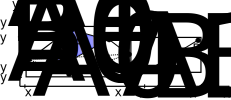
\includegraphics[width=0.7\textwidth]{pics/pdf/ccd_aabb.pdf}
  \caption[2D Illustration of  AABB to accelerate CCD by example of a triangle and a vertex.]{2D Illustration of  AABB to accelerate CCD by example of a triangle and a vertex. The arrows indicate the trajectory of the vertices within the time step. The boxes surrounding the features are the according AABB. The minimum and maximum coordinates for both AABB are consecutive in the x-direction. Therefore, there is no intersection.}
  \label{fig:ccd_aabb}
\end{figure}
To test for intersections between two AABB, the minimum and maximum values for each axis are sorted in ascending order. As long as for at least one axis the minimum and maximum coordinates for both AABB are consecutive there is no intersection. Otherwise, the AABB intersect and the elementary test needs to be applied.

We do not apply a hierarchical order of the AABB, as it is common used for bounding volume hierarchies \cite{TESCHNER2005}.

